
\chapter{Validierung}

Im folgenden Kapitel wird die Deformationerkennung validiert.
Zur Überprüfung werden Materialeigenschaften und aufgenommene Messwerte 
mit der erkannten Deformation verglichen.

\section{Messergebnisse} \label{validation}

Es wurden fünf Bauteile mit verschiedenen Spannungsstufen gemessen. Für jede 
Spannungsstufe wurde die Kraft, die auf das Bauteil wirkte sowie die Verschiebung 
des Schraubstocks gemessen.
Jede Spannungsstufe wurde durch Schrittweises anziehen des Schraubstocks erreicht.
Die Spannkraftkurve eines einzelnen Einspannvorgangs ist in 
Abbildung \ref{fig:single} zu sehen. 
In der Spannungskurve ist ein elastischer Bereich für das 
Bauteil zu sehen, in dem sich die Spannkraft zurückbewegt, nachdem kein 
Anzugdrehmoment mehr anliegt. Für die Validierung ist, die maximal anliegende 
Spannkraft von Interesse. Auf Grund der Elastizität kann nicht der maximal vorliegende 
Wert der Spannkraft angenommen werden, 
sondern es muss ein Wert gewählt werden der nach dem maximalen Ausschlag liegt.
Dieser wurde über die erste Ableitung der Spannkraftkurve ermittelt. Sobald der 
Absolutwert der Steigung unter 0.0009 N fällt, wir die Spannkraft und Auslenkung an 
diesem Punkt gewählt. 0.0009 N wurde empirisch ermittelt, um bei allen Bauteilen einen 
angemessenen Wert zu liefern.
Die Spannkraft wurde an zwei Achsen gemessen und zu einer Gesamtkraft aufsummiert.

\begin{figure}[H]
    \centering
    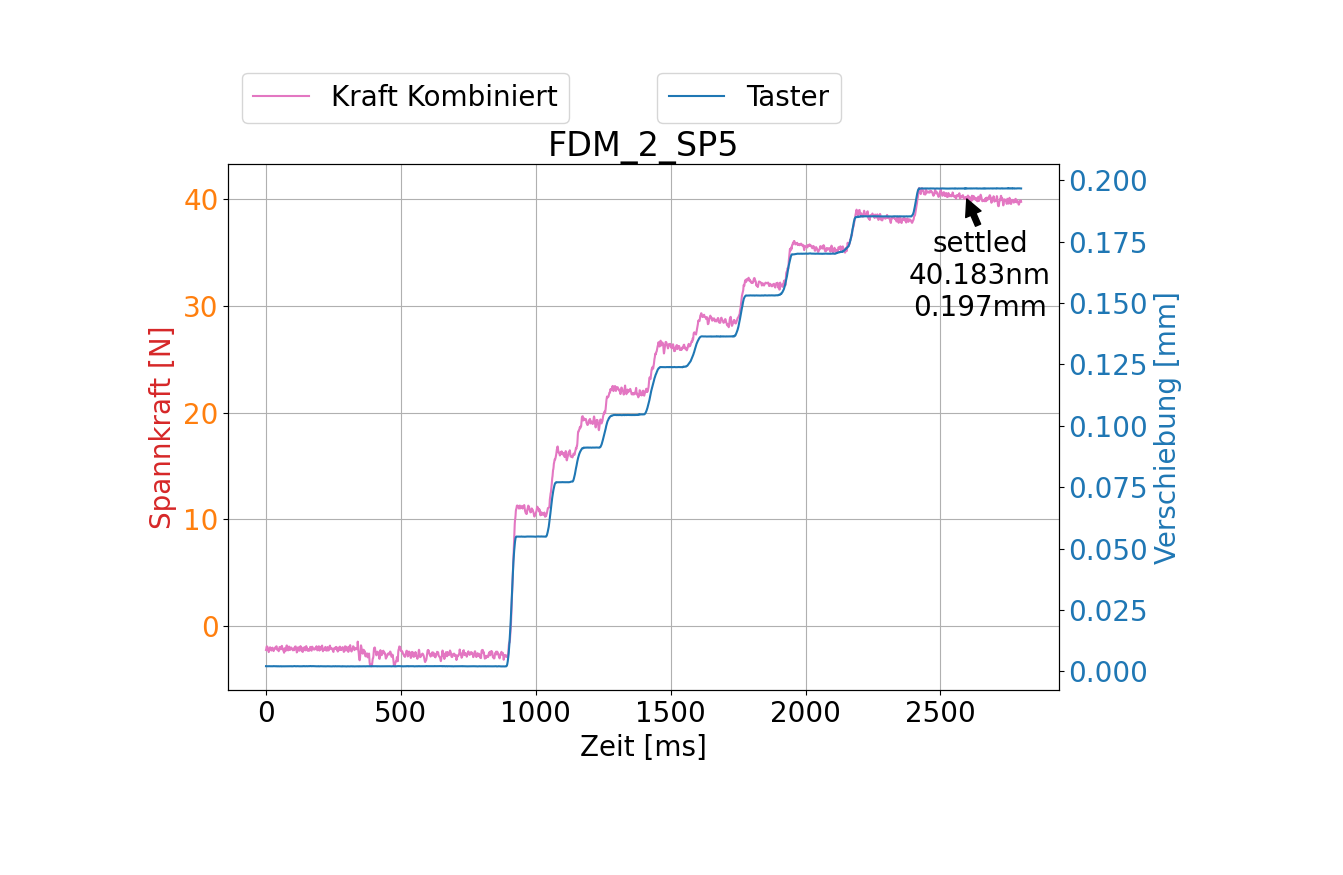
\includegraphics[width=0.99\textwidth]{images/spannkraftstufen_single.png}
    \caption{Kraft, die auf ein FDM Bauteil wirkt, während es angezogen wird. In diesem 
    wurde von Spannungsstufe vier auf Spannungsstufen fünf erhöht. Zusätzlich ist 
    die Verschiebung der Backen dargestellt.}
    \label{fig:single}
\end{figure}

Diese maximalen Werte für die Spannkraft und Auslenkung wurden für jedes Bauteil 
akkumuliert und sind in Abbildung \ref{fig:akkumulated} dargestellt. 
Die mit dem FDM-Prozess hergestellten Bauteile wurden jeweils in sechs Spannungsstufen
gemessen. Zwischen den Stufen wurde versucht, eine konstante Kraft auf das Bauteil 
auszuüben. Durch den manuellen Prozess des Anziehens des Schraubstocks war dies 
jedoch nicht immer möglich.
Die Metallbauteile unterscheiden sich durch ihren Aufbau. 
Alle basieren auf dem gleichen 3D-Modell, besitzen jedoch unterschiedliche 
Stützstrukturenanteile. Im Bauteil AM0 ist die vollständige Stützstruktur vorhanden,
während in den Bauteilen AM1 und AM2 die Stützstruktur in unterschiedlicher 
Tiefe ausgebohrt wurde. Die Bauteile sind in Abbildung \ref{fig:am_parts} dargestellt.

Das Bauteil AM0 wurde nur mit zwei Spannungsstufen gemessen, 
da bereits bei der zweiten Stufe über 2500 N Kraft erforderlich war, 
um das Bauteil nur minimal in x-Richtung zu deformieren. Dies zeigt, 
dass die Stützstruktur einen erheblichen Einfluss auf die Verformbarkeit 
eines Bauteils hat. Bei Bauteil AM1 wurden 2500 N erst nach vier Spannungsstufen 
erreicht.

Die FDM-Bauteile wurden mit deutlich weniger Kraft eingespannt. 
Hier wurde bei etwa 250 N gestoppt, dennoch ist die Verschiebung der 
Teile deutlich größer als bei den Metallbauteilen. Diese Werte wurden aufgenommen, 
um die visuelle Deformationserkennung zu validieren. In Abbildung \ref{fig:akkumulated} 
ist die Spannkraft und Verschieben der fünf Demonstratorbauteile dargestellt.

\begin{figure}[H]
    \centering
    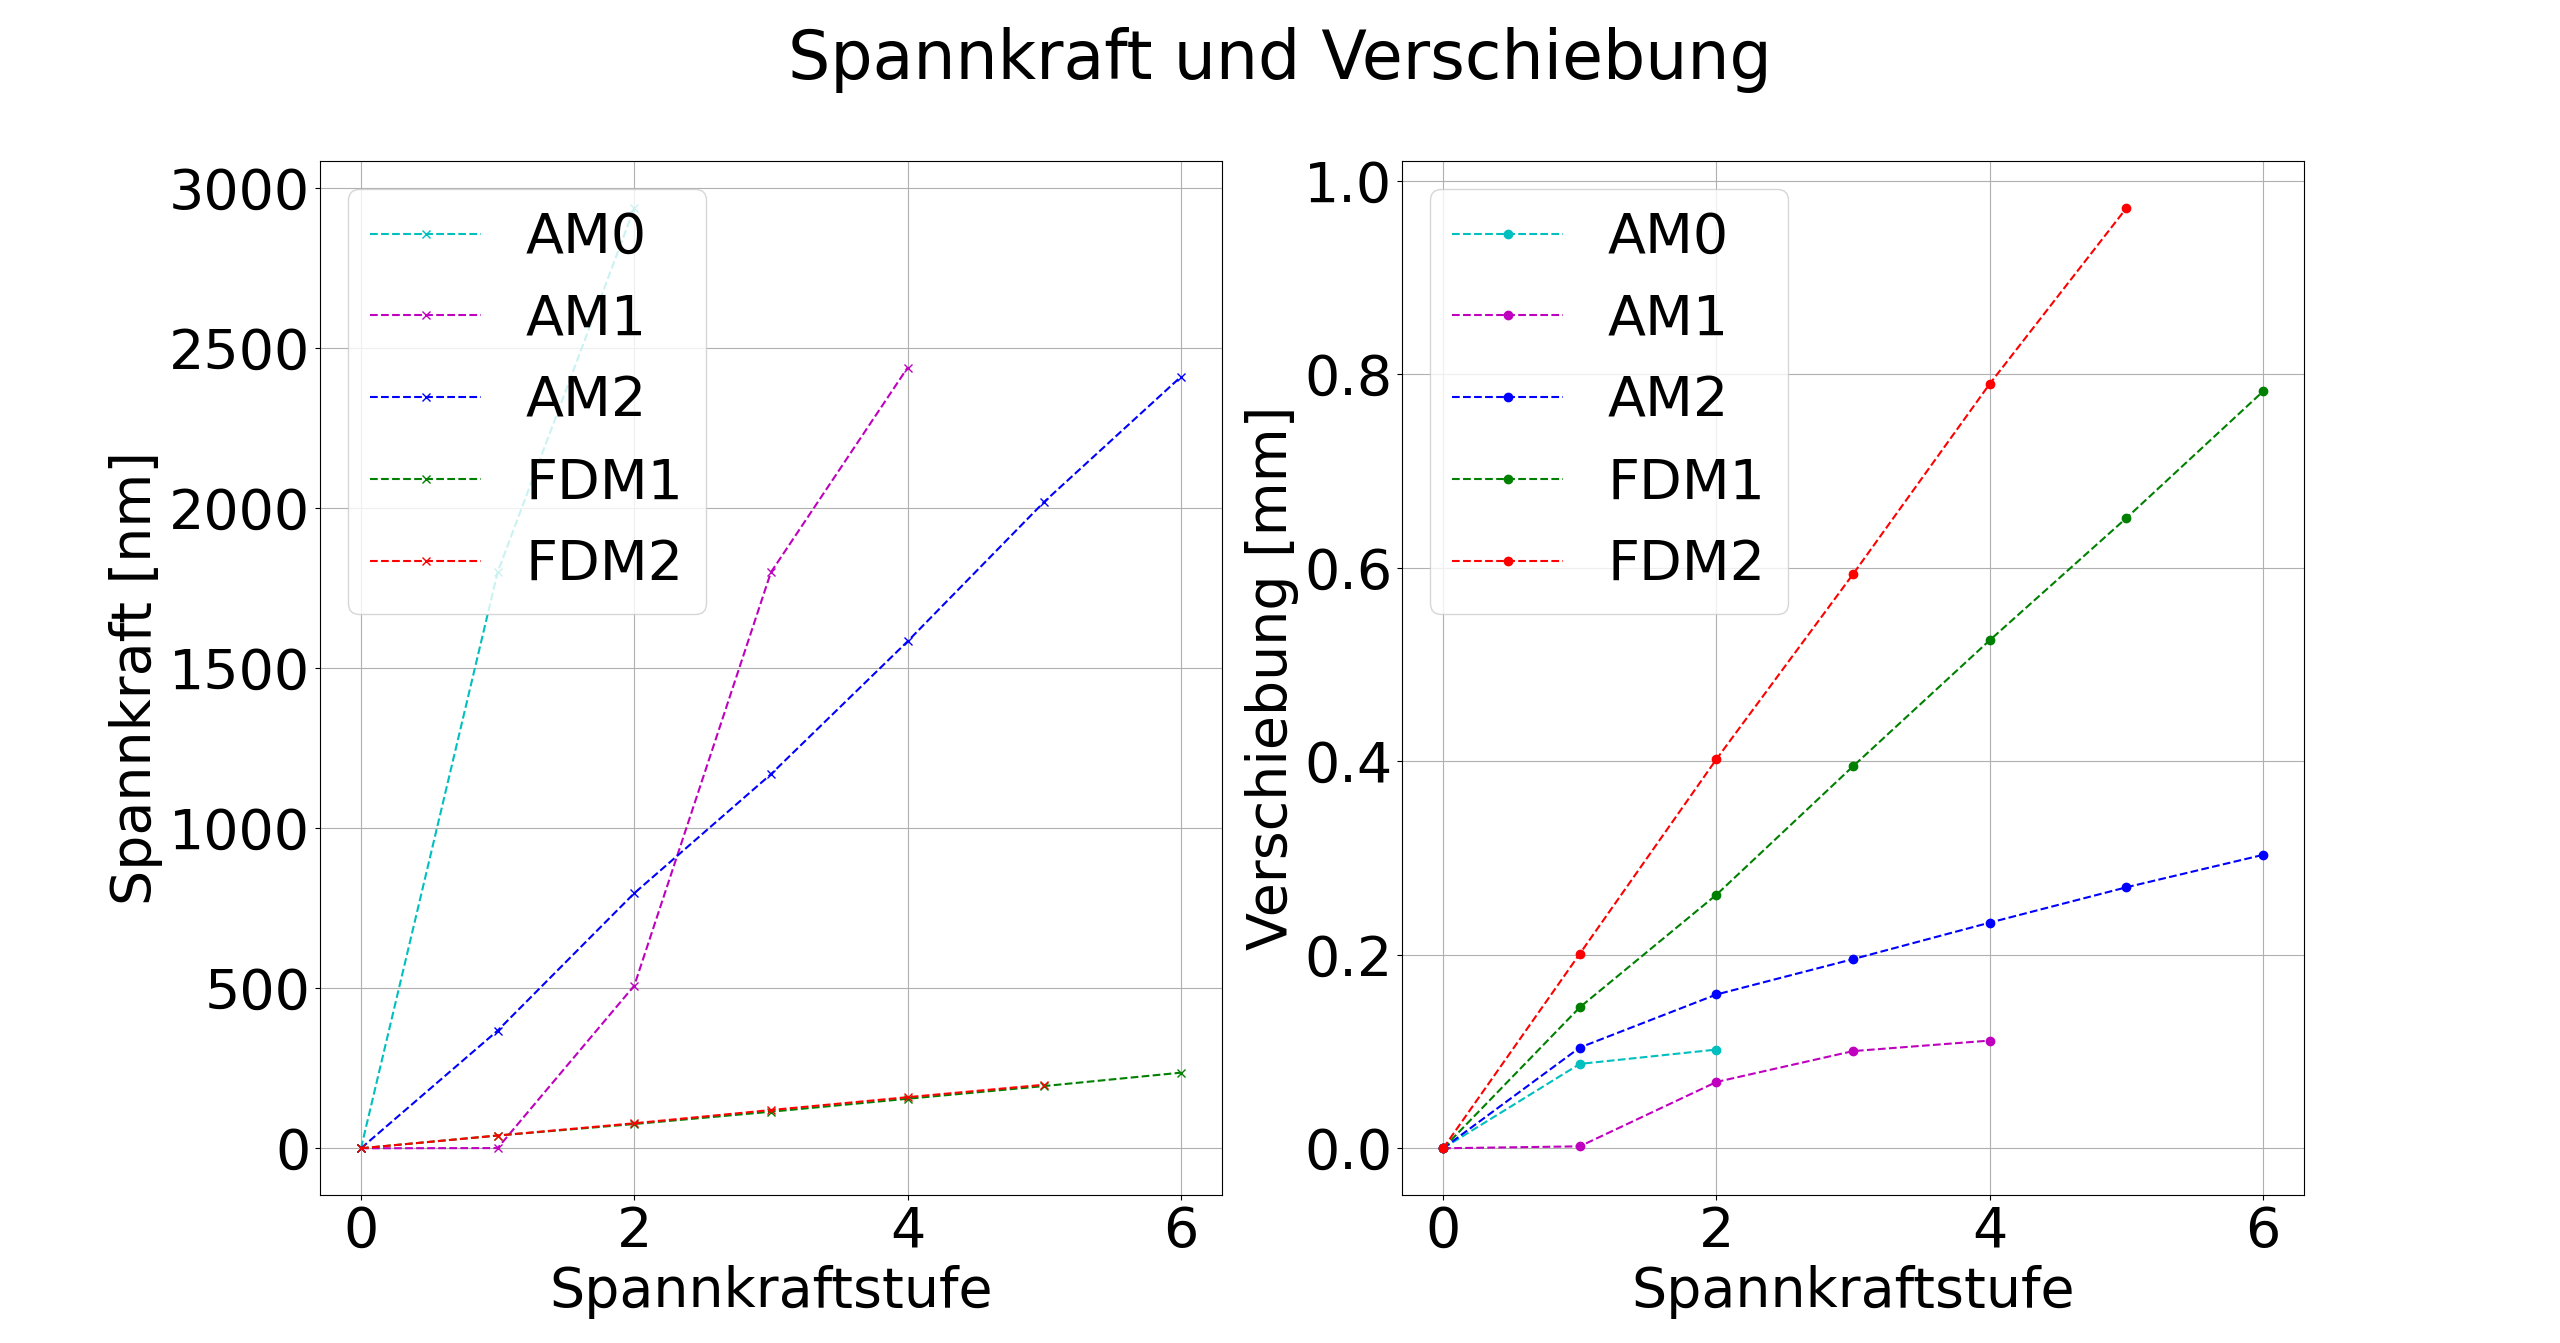
\includegraphics[width=0.99\textwidth]{images/spannkraftstufen_akkumuliert.png}
    \caption{Akkumulierte Kraft und Verschiebung, mit der jedes Bauteil deformiert wurde.}
    \label{fig:akkumulated}
\end{figure}

\begin{figure}[H]
    \centering
    \begin{minipage}{.33\textwidth}
      \centering
      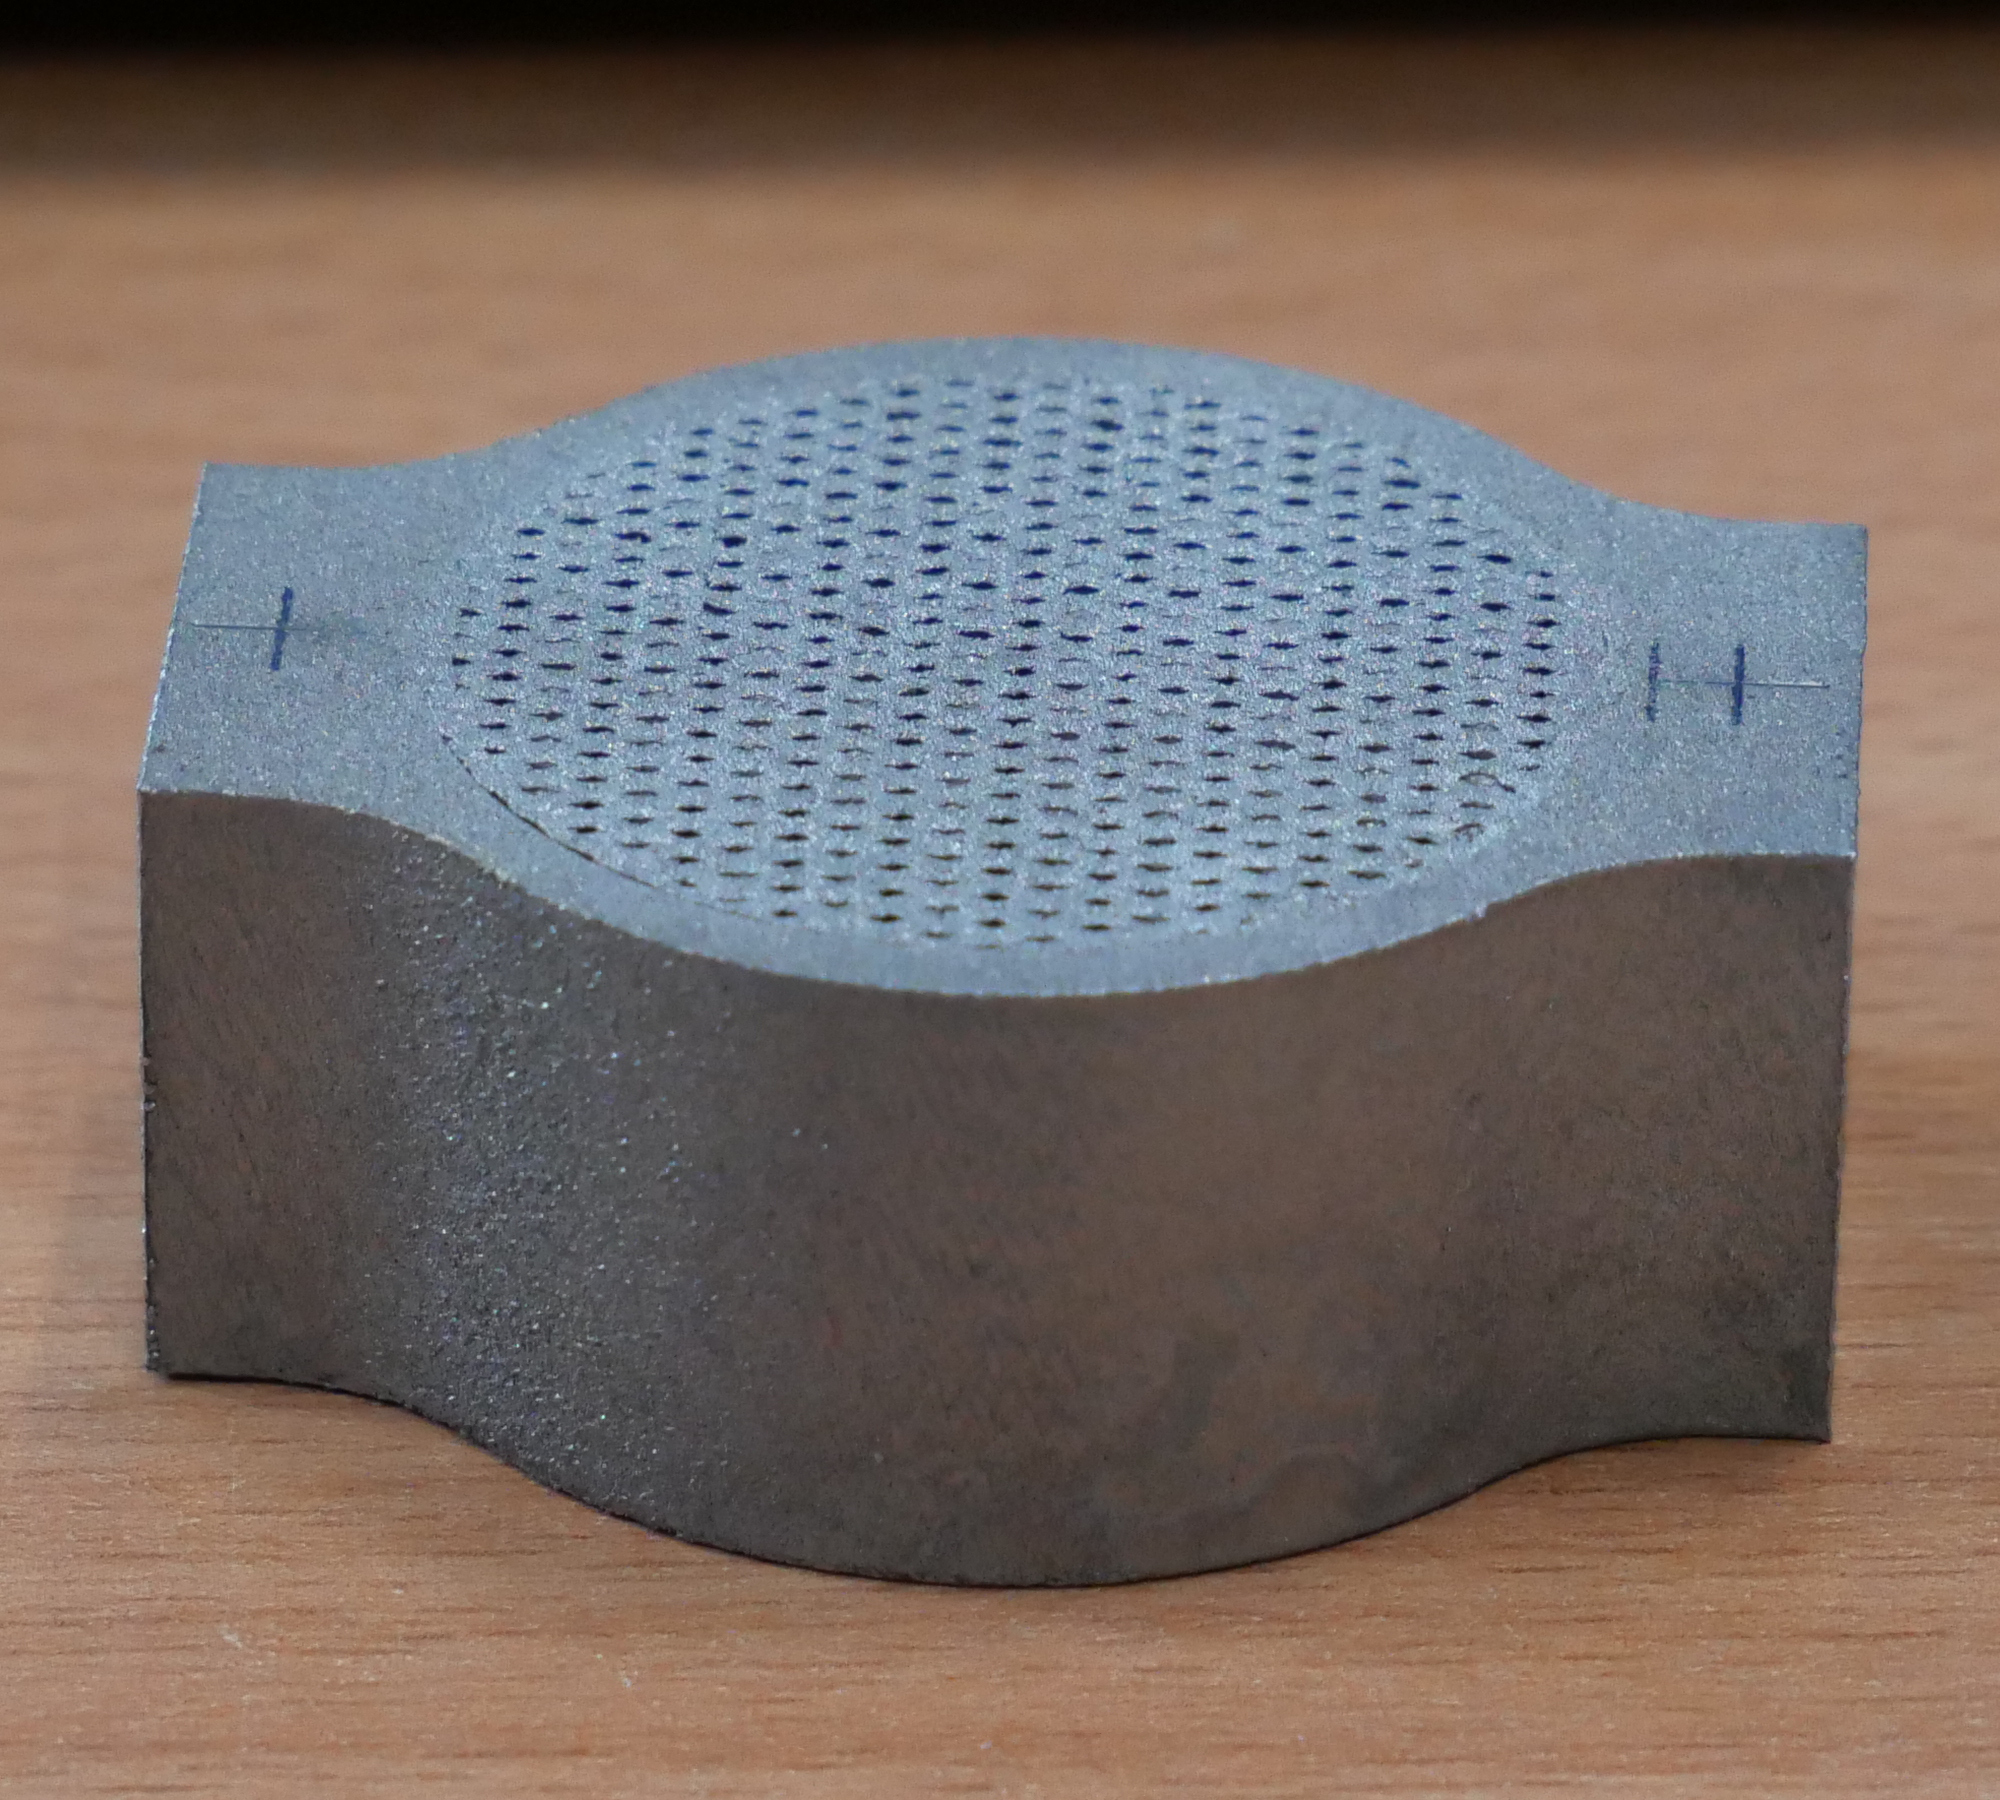
\includegraphics[width=0.9\linewidth]{images/AM0_crop.JPG}
      \caption*{(a)}
    \end{minipage}%
    \begin{minipage}{.33\textwidth}
      \centering
      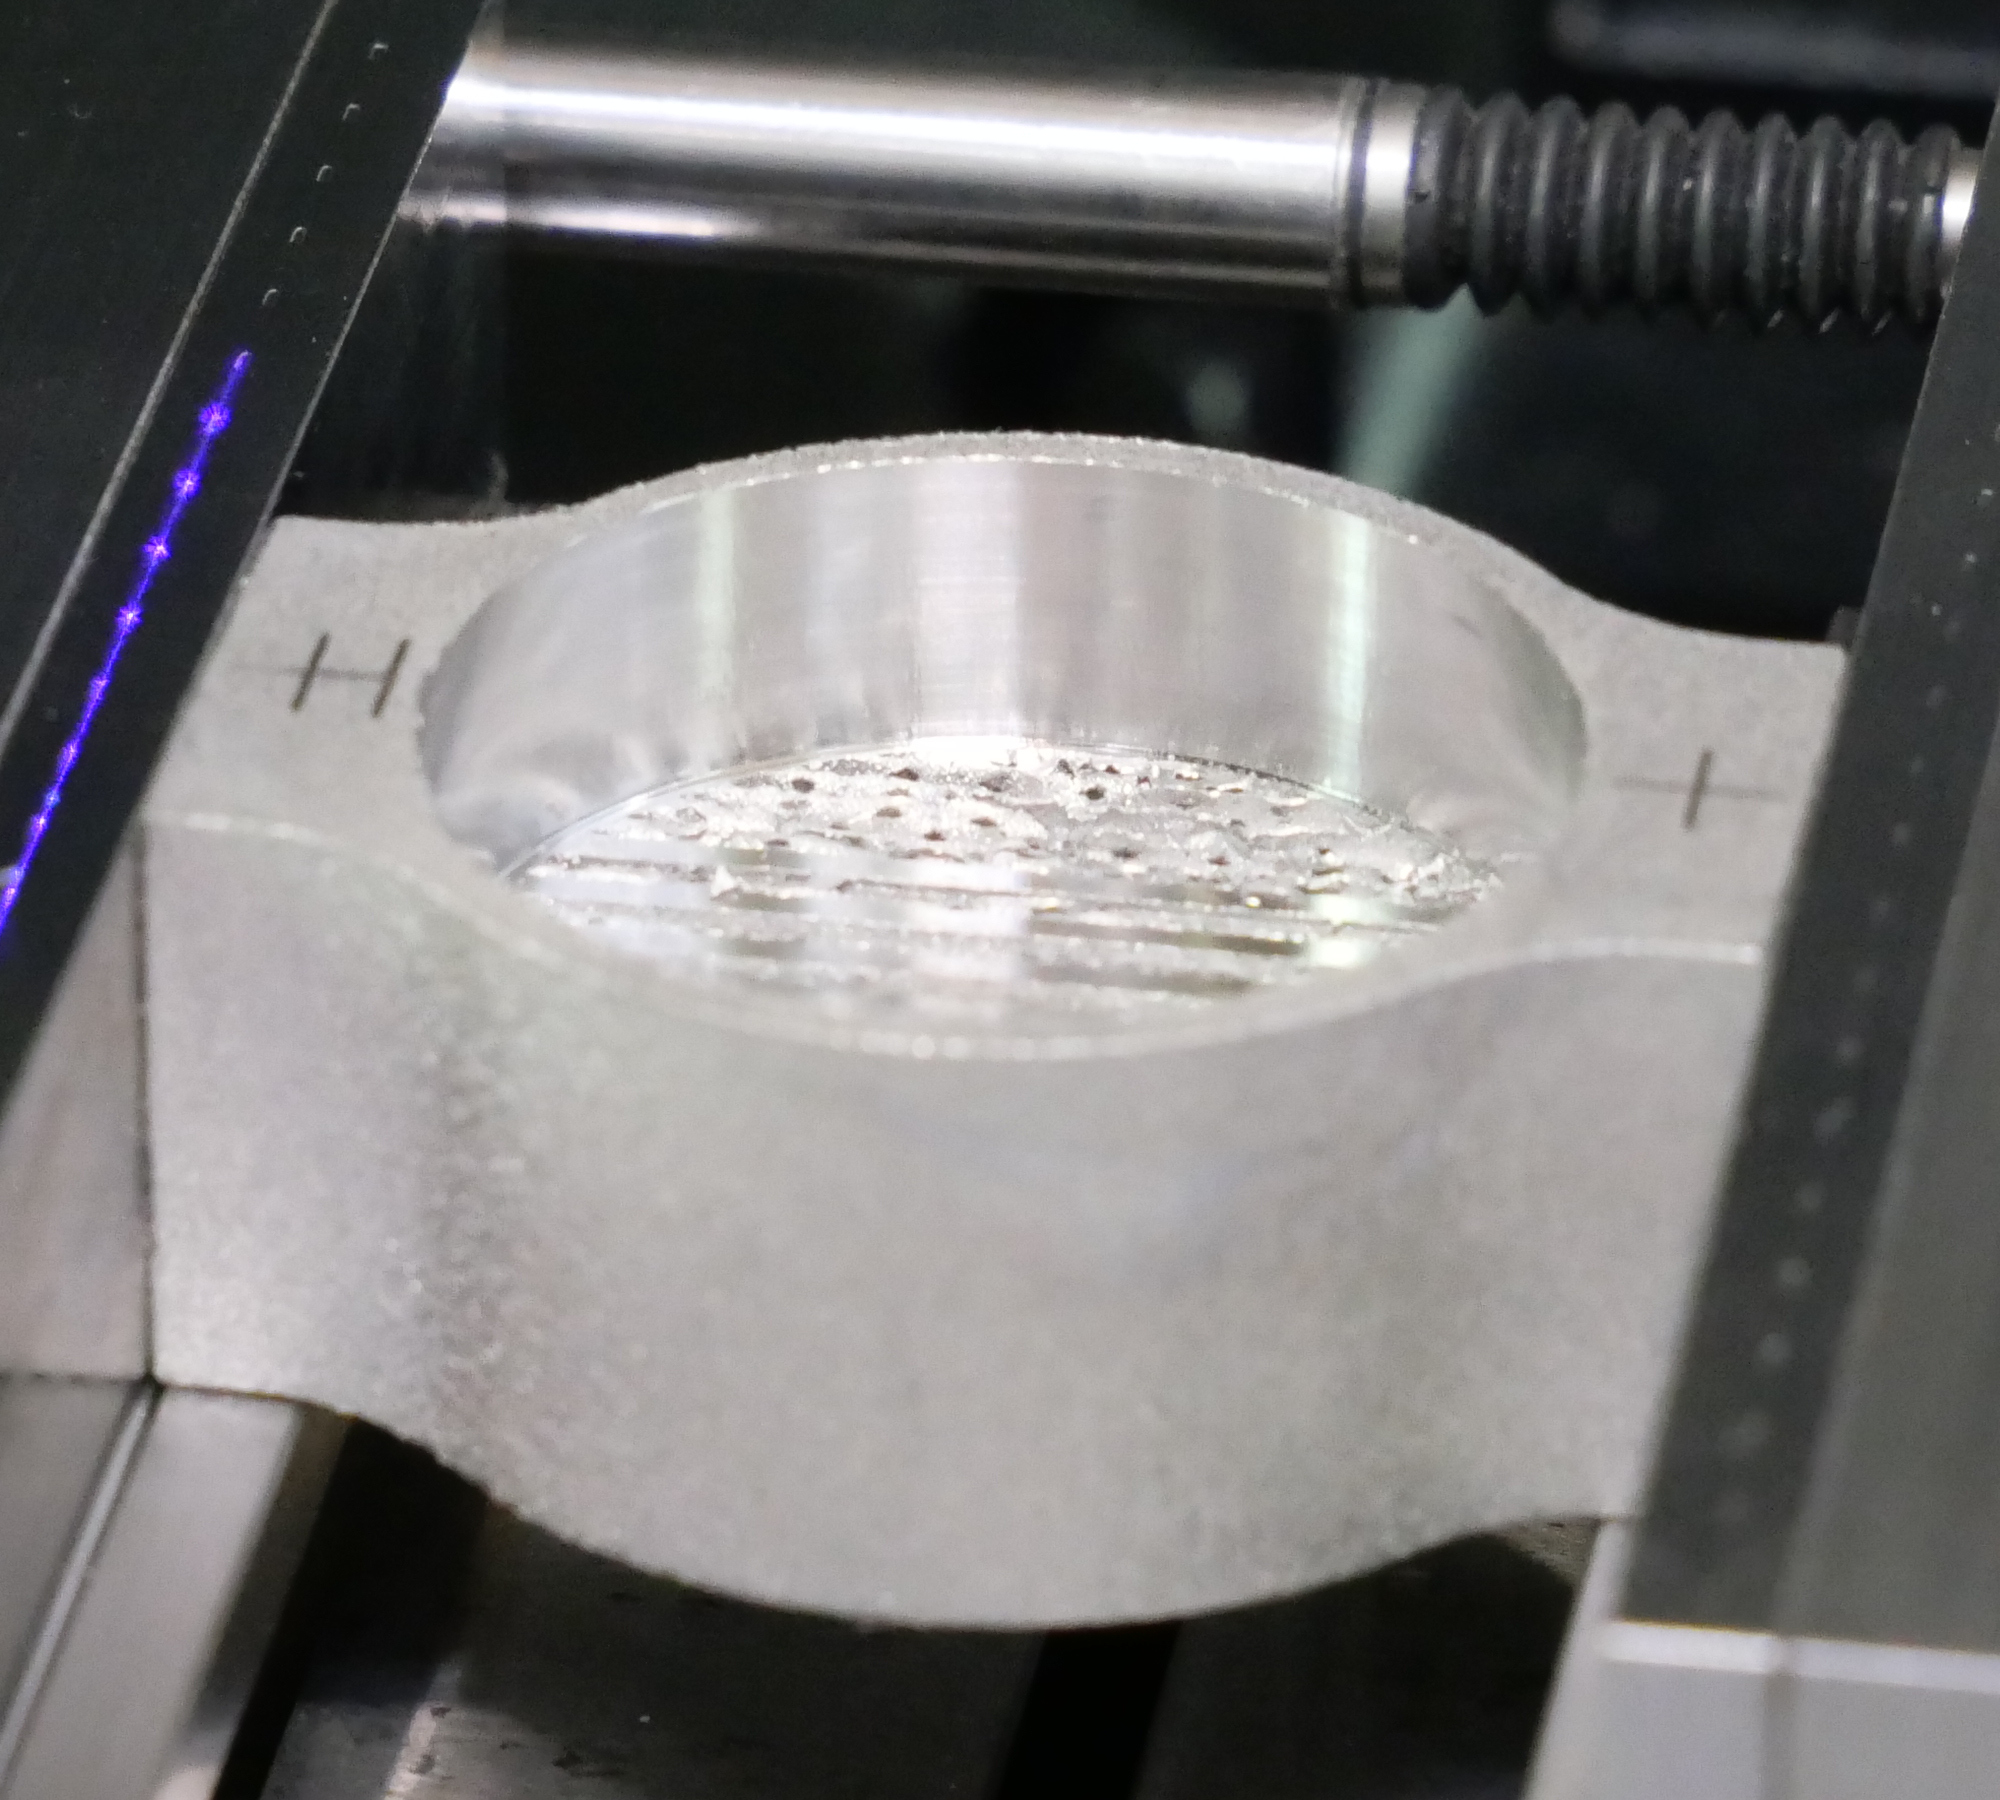
\includegraphics[width=0.9\linewidth]{images/AM1_crop.JPG}
      \caption*{(b)}
    \end{minipage}
    \begin{minipage}{.33\textwidth}
        \centering
        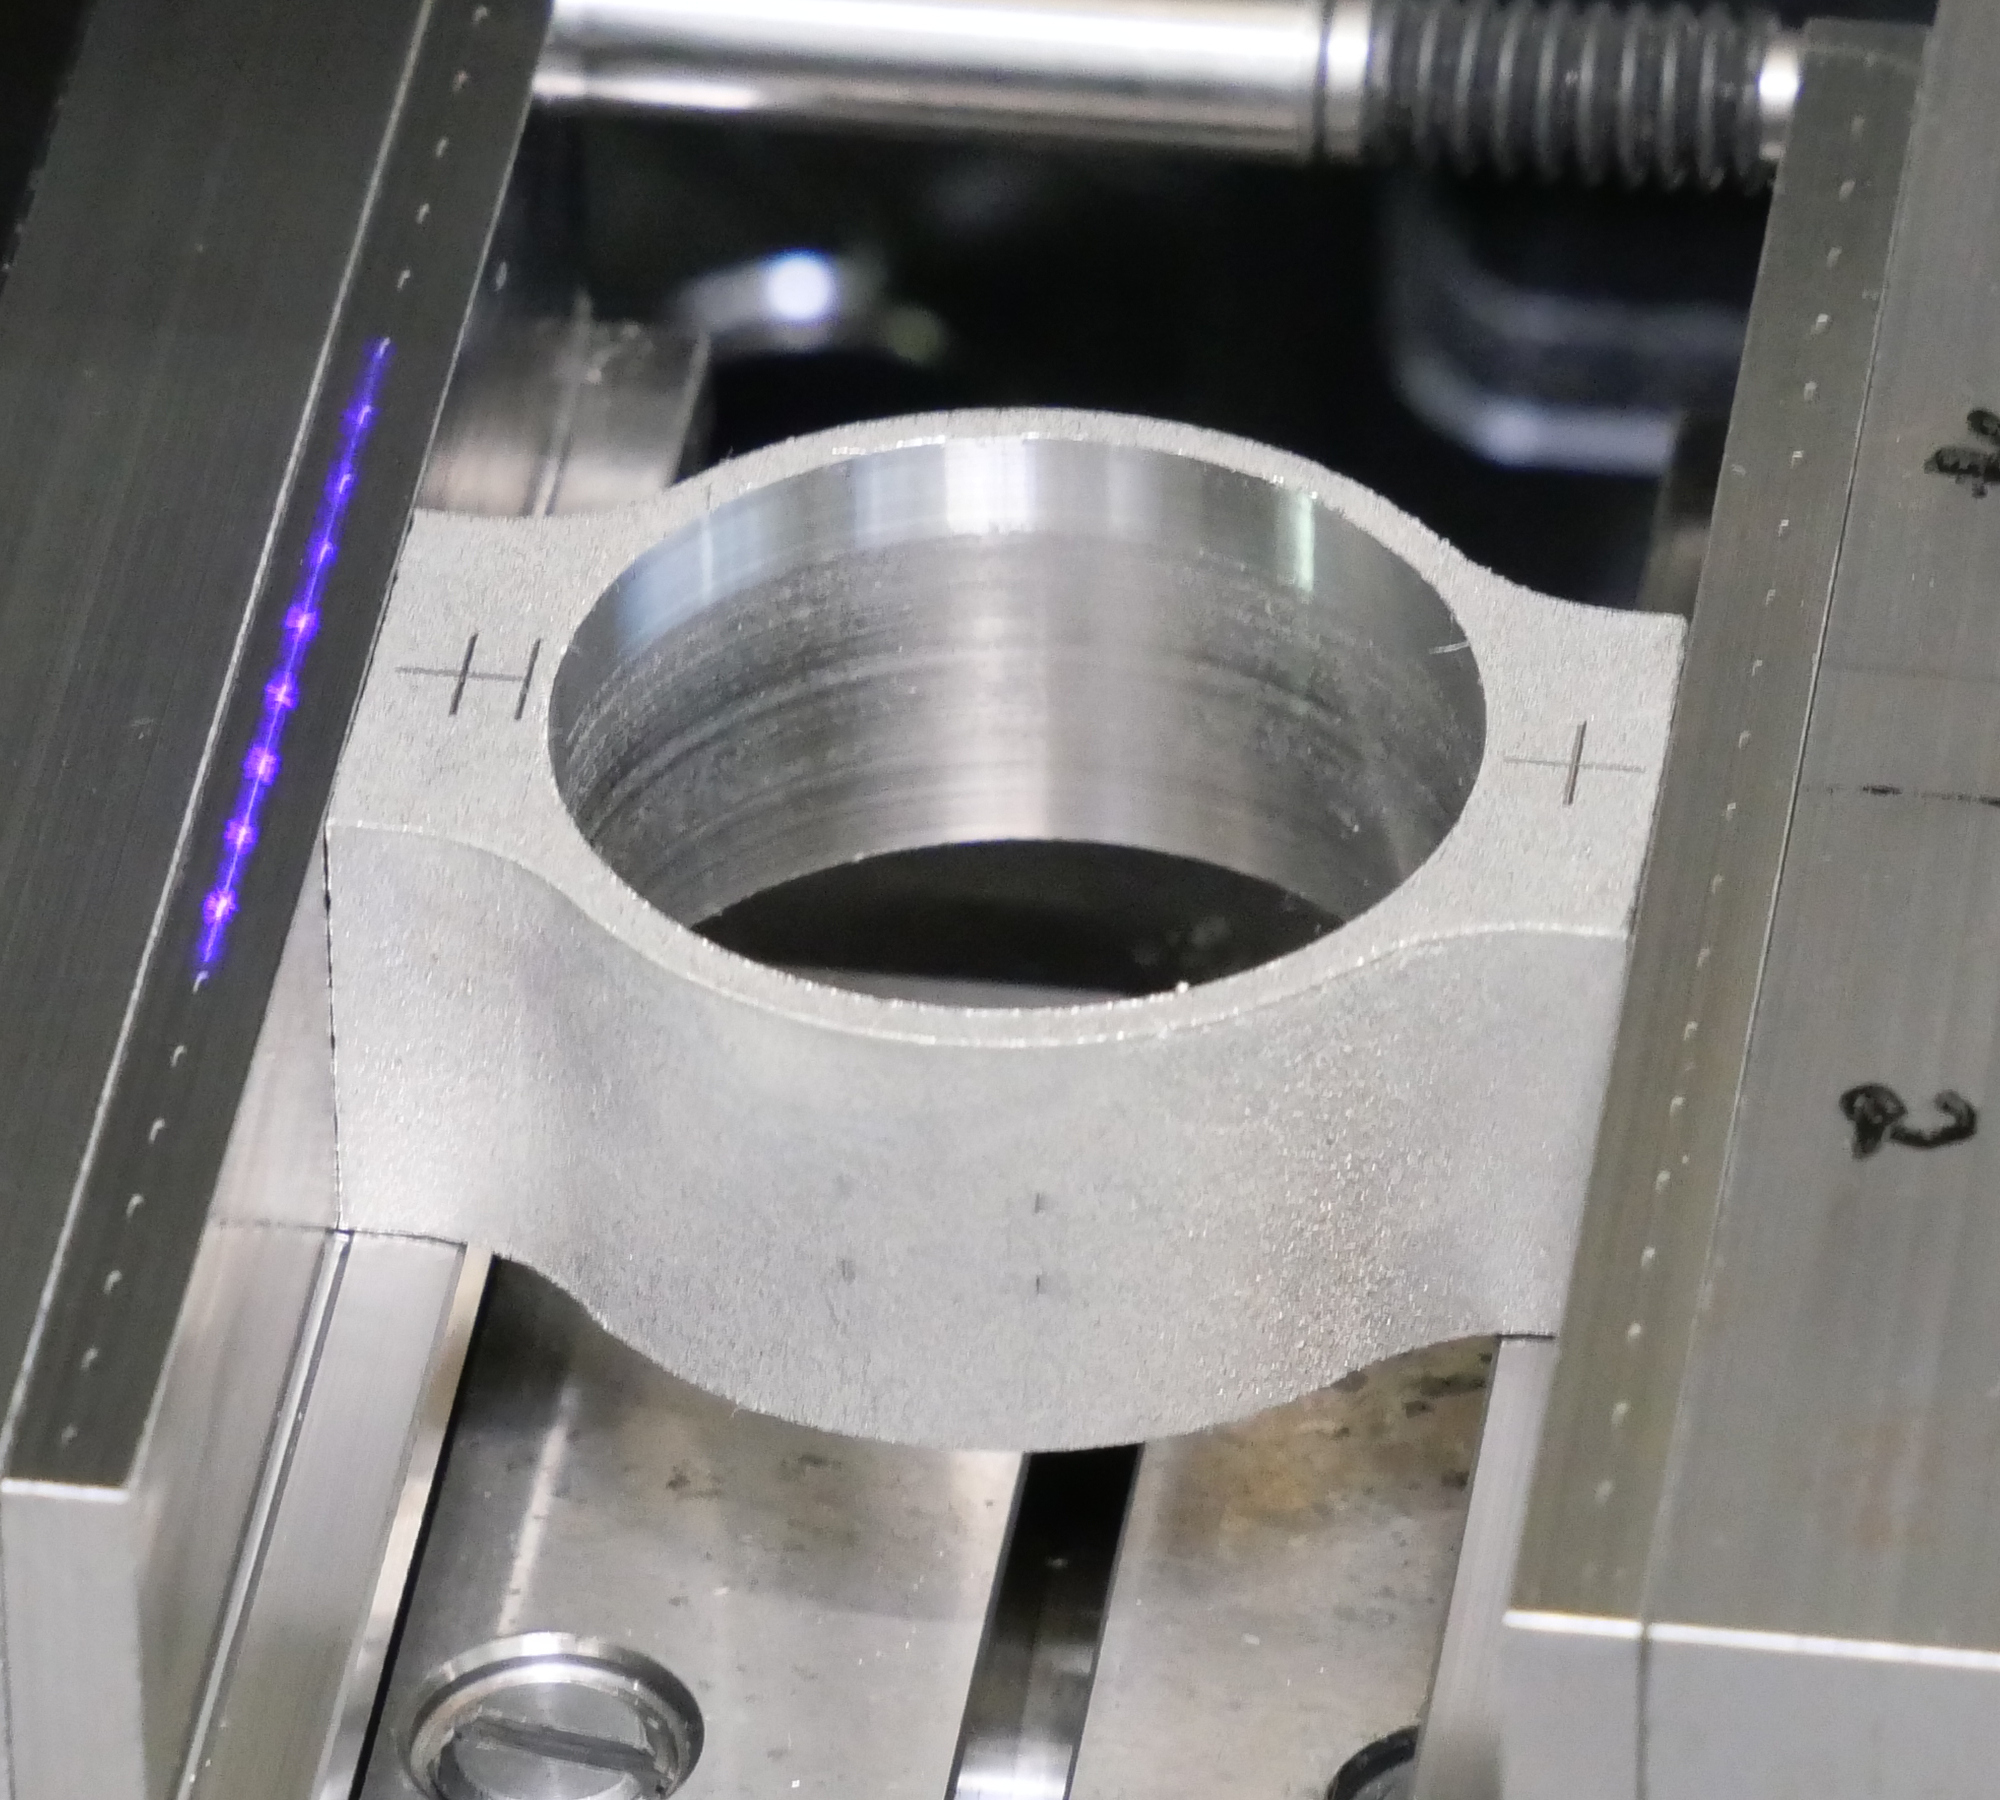
\includegraphics[width=0.9\linewidth]{images/AM2_crop.JPG}
        \caption*{(c)}
      \end{minipage}
      \caption{(a): AF Metallbauteil mit voller Stützstruktur, Bezeichnung: AM0.
      (b): AF Bauteil mit der halben Stützstruktur ausgebohrt, Bezeichnung: AM1.
      (c): AF Bauteil ohne Stützstruktur, Bezeichnung: AM2}
      \label{fig:am_parts}
\end{figure}

\section{Ergebnisse der optischen Deformationsanalyse} \label{defodata}

In Abbildung \ref{fig:am_defos} und Abbildung \ref{fig:fdm_defos} sind die erkannten
Deformation dargestellt. Jeweils von Spannungsstufe null bis 
Spannungsstufen Sechs. Bei dem FDM Bauteil fehlt die Spannungsstufen fünf, 
diese ist leider bei der händischen Dateiname Vergabe überschrieben worden und konnte 
deshalb nicht ausgewertet werden. Aus diesem Grund ist eine so große Lücke in der 
Abbildung \ref{fig:fdm_defos} zu sehen.
Außerdem sind große Unterschiede in den y-Werten der Deformation zu sehen. Zum Beispiel 
die rote Kurve in Abbildung \ref{fig:am_defos}, die den Unterschied der Spannungsstufen 
null und eins angibt, liegt deutlich über den anderen Kurven. 
Diese Kurve sollte näher an null der y-Achse liegen. 
Dies liegt an Ungenauigkeiten in dem Stitching Verfahren. In den Graphen ist mehr 
auf die Steigung der Deformationskurve zu achten und weniger auf ihre Position.
In der Steigung ist zu erkennen, dass
sich die Bauteile im mittleren Bereich nach am stärksten nach außen hin deformiert haben.
Außerdem ist im Vergleich der beiden Graphen (Abb. \ref{fig:am_defos} und \ref{fig:fdm_defos}) 
zu sehen, dass sich das FDM Bauteil deutlich mehr, als das Metallteil, verformt hat. 
Hier beträgt die größte Deformation über 150 Pixel.
Bei dem Metallbauteil, das mit der zehnfachen Kraft eingespannt wurde (250 nm vs. 2500 nm)
sind es nur knapp 40 Pixel, wie in Abbildung~\ref{fig:am_defos} zu sehen ist.
Trotzdem ist zu sehen das sich die Bauteile, die auch die 
gleiche Geometrie teilen, auf die gleiche Weise verformt haben.
Bei dem Metallbauteil mit Stützstruktur ist zu sehen, dass es sich anders 
verformt. In Abbildung \ref{fig:deformation_data_am} ist zu erkennen, dass 
die maximale Deformation nicht in der Mitte liegt wie bei den vorherigen Bauteilen, 
sondern das Bauteil linear verformt wird. Hier sehen beide Deformationskurven aus, 
wie sie erwartet werden. Diese Graphen stimmen folglich mit dem erwarteten Verhalten überein.

\begin{figure}[H]
  \centering
  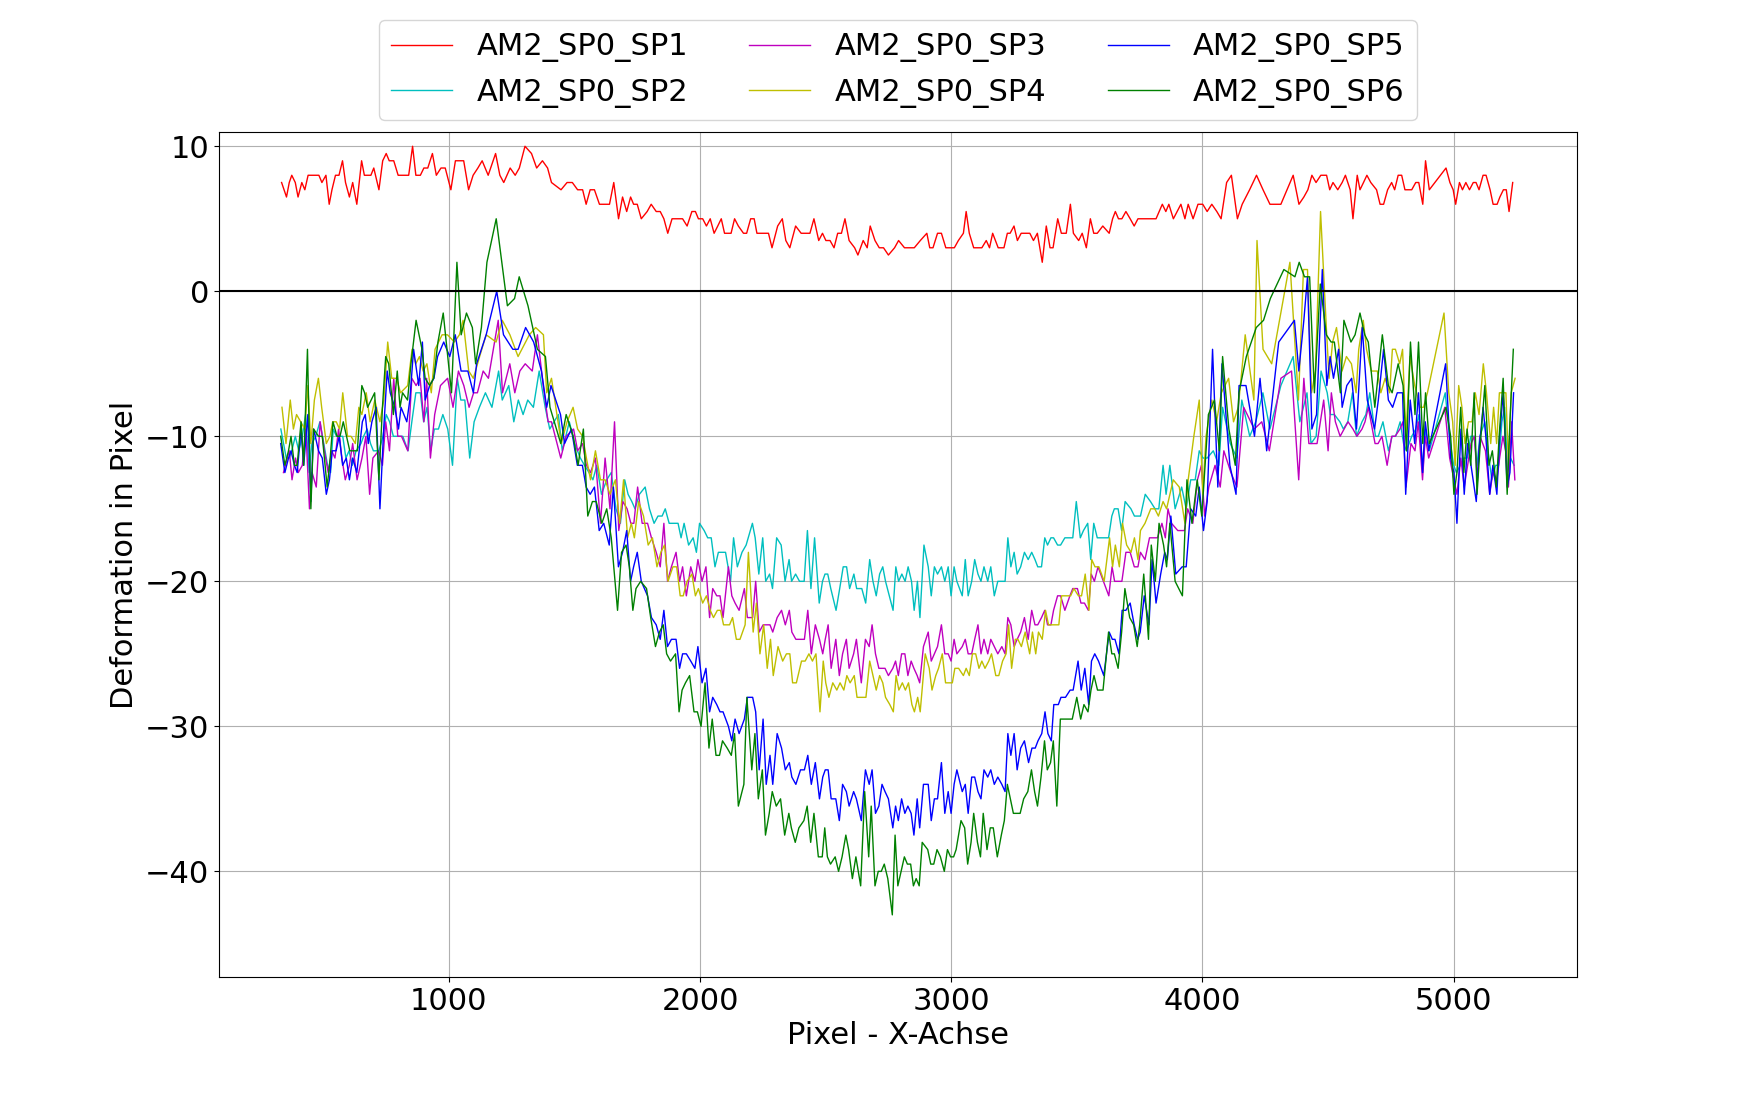
\includegraphics[width=0.95\textwidth]{images/am2_all_defos.png}
  \caption{Sechs Deformationsstufen bei einem additiv gefertigten Metallbauteil ohne
  Stützstruktur von 0 bis 2500 nm}
  \label{fig:am_defos}
\end{figure}

\begin{figure}[H]
  \centering
  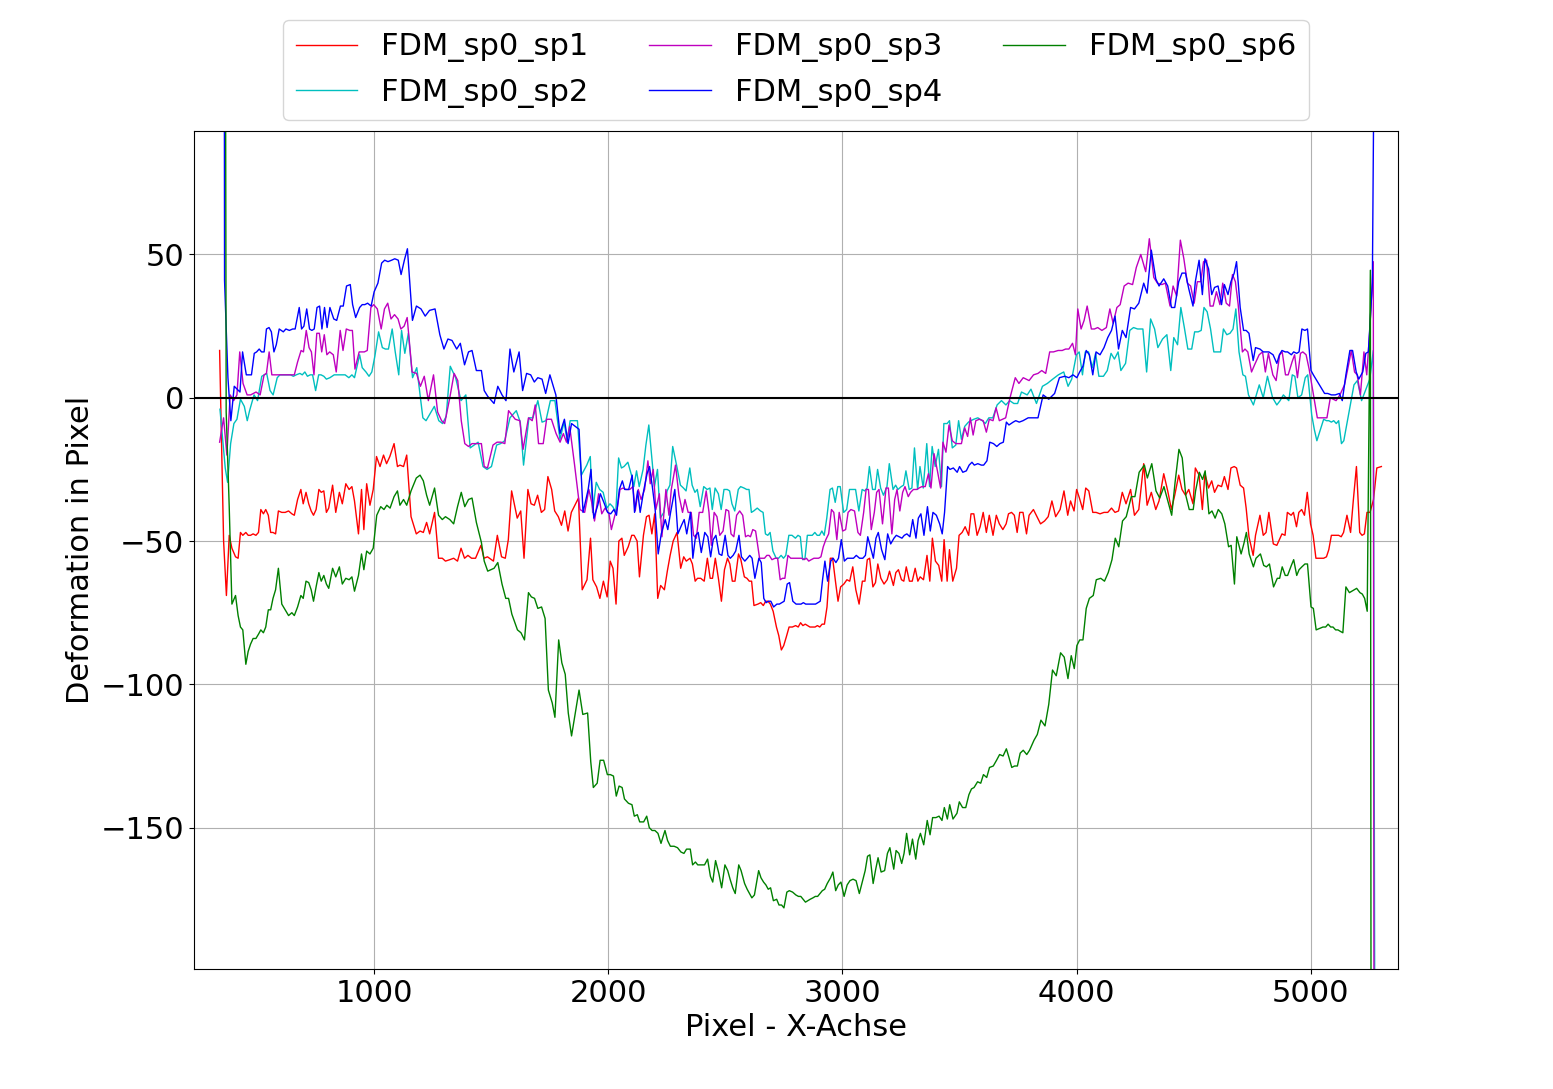
\includegraphics[width=0.95\textwidth]{images/fdm2_all_defos.png}
  \caption{Fünf Deformationsstufen bei einem FDM Bauteil von 0 bis 250 nm}
  \label{fig:fdm_defos}
\end{figure}

\begin{figure}[H]
    \centering
    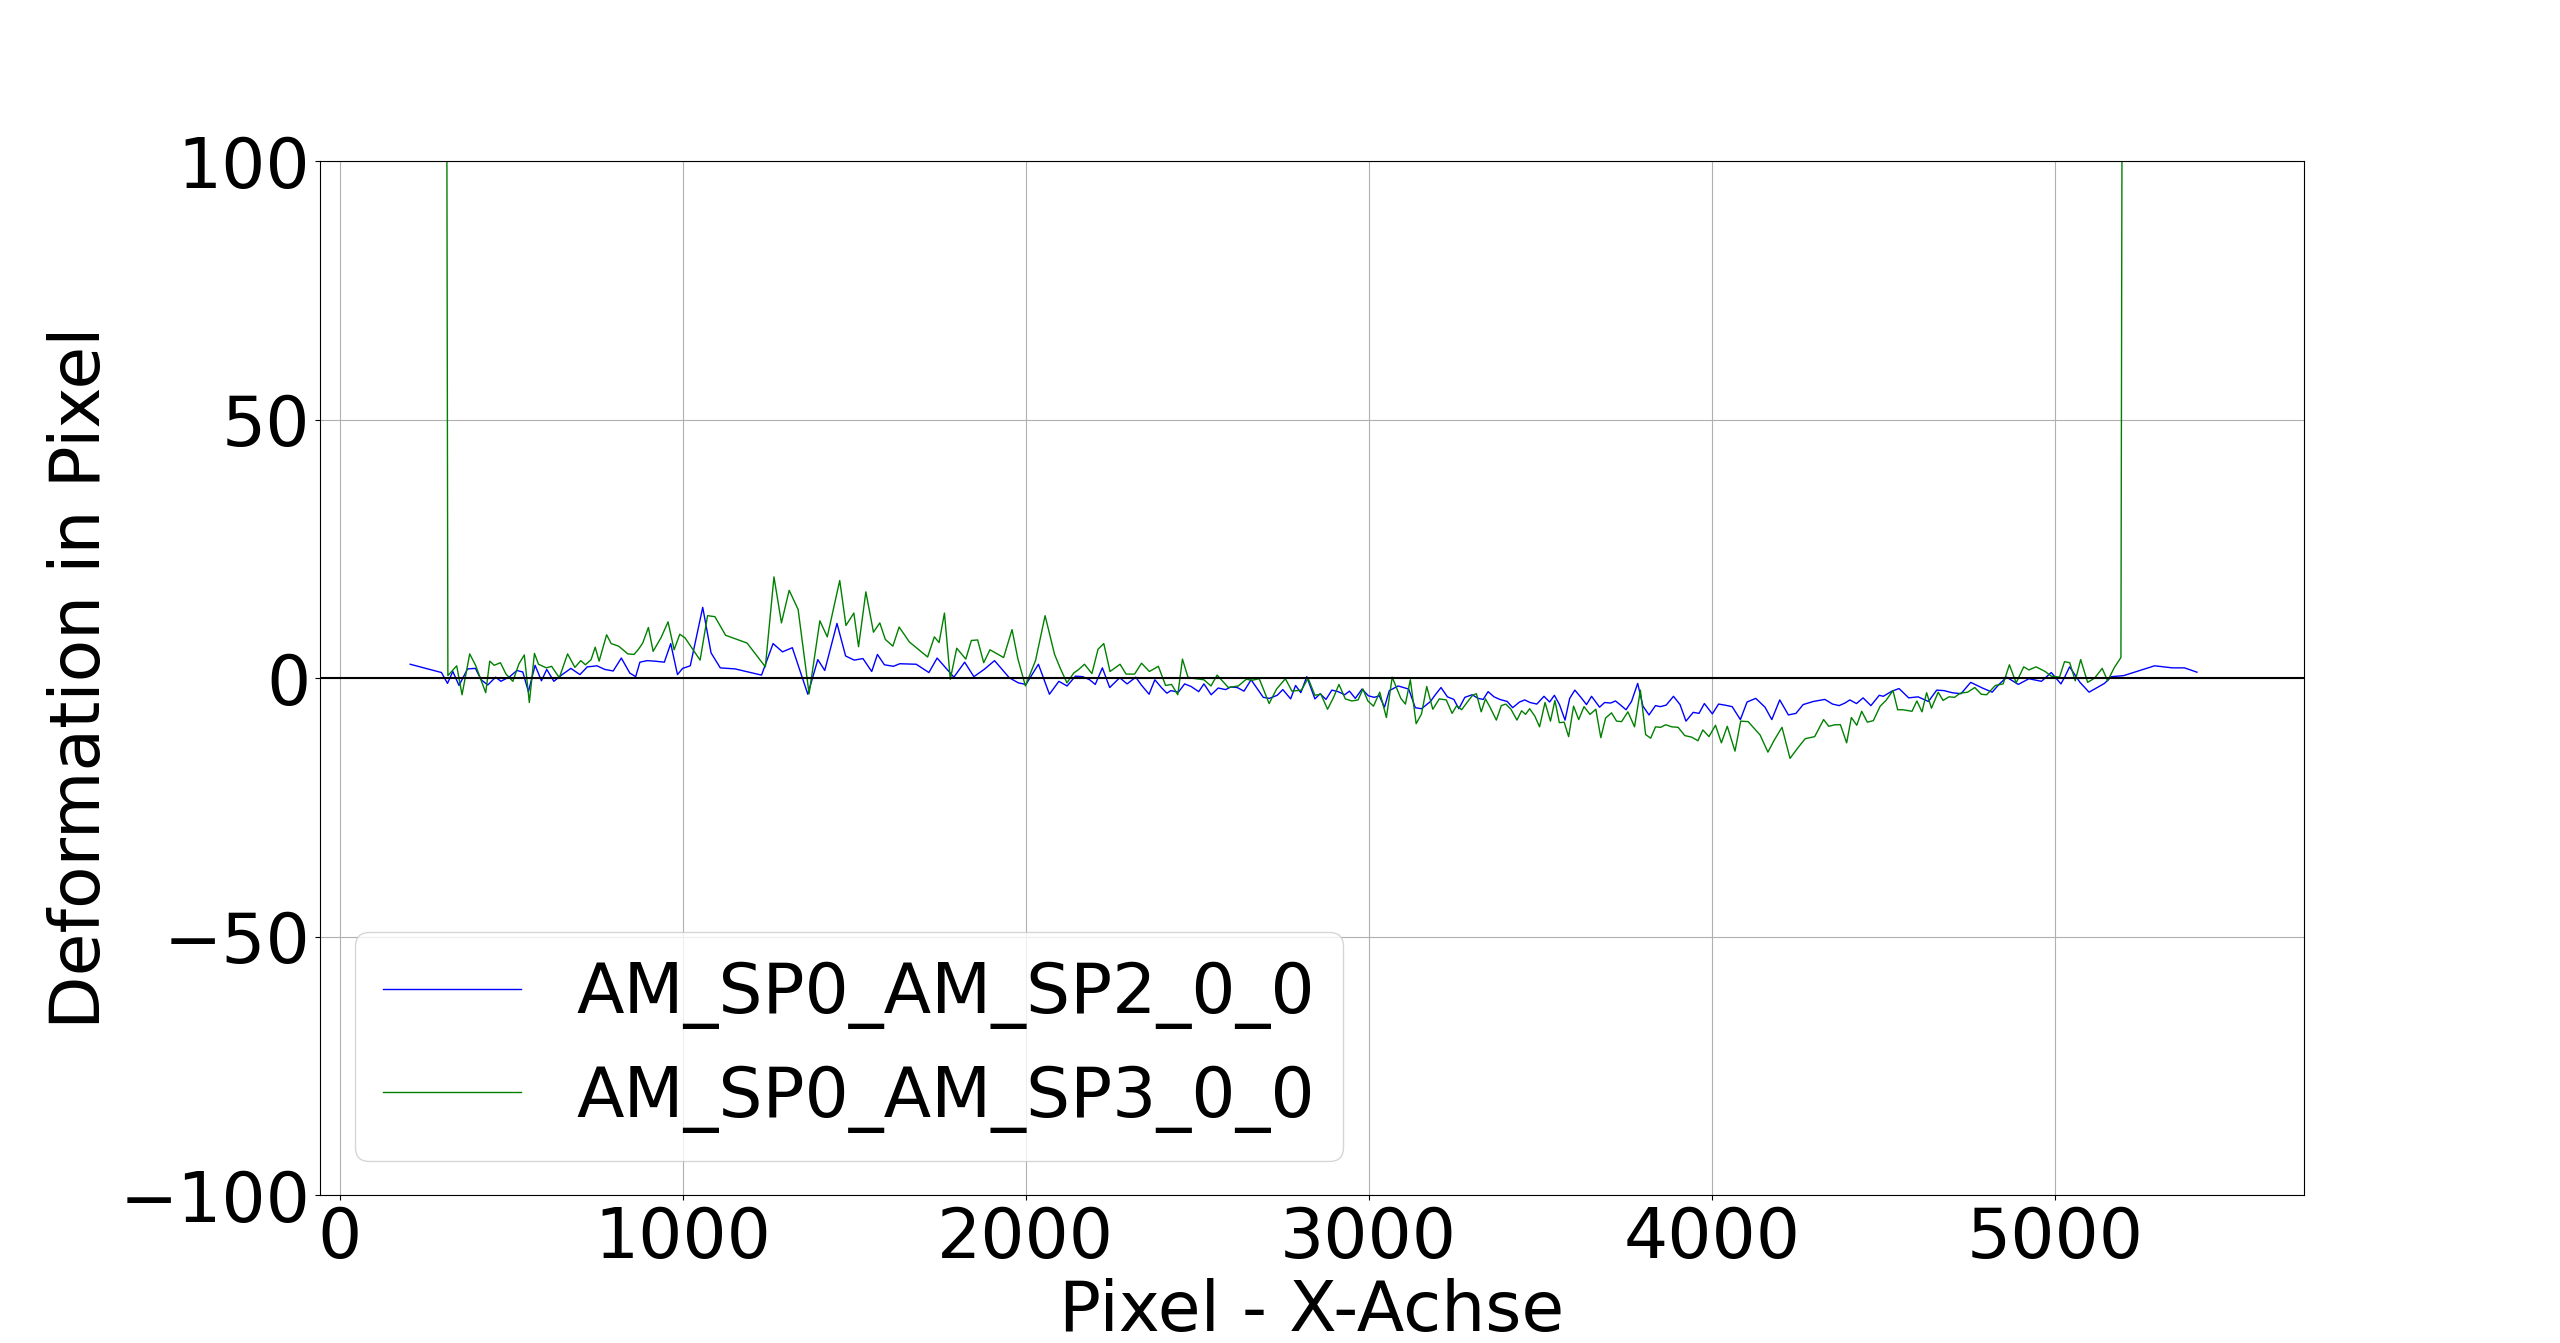
\includegraphics[width=0.9\textwidth]{images/AM_sp0_sp2_defo_plot.png}
    \caption{Differenz von zwei Spannungsstufen bei einem additiv gefertigten Metallbauteil, 
    das zur Hälfte mit Stützstrukturen gefüllt ist (Abbildung~\ref{fig:am_parts} (b)). }
    \label{fig:deformation_data_am}
\end{figure}

\section{Beurteilung der Ergebnisse}

Grundsätzlich ermöglicht die Methode die Erkennung und den Vergleich von Deformationen 
eines Bauteils. Die gemessenen Deformationen eines Bauteils entsprechen den erwarteten Werten, 
abhängig von Material und Geometrie des Bauteils. FDM-gedruckte Kunststoffteile zeigen 
eine deutlich stärkere Verformung im Vergleich zu Metallteilen.
Bei den Metallteilen zeigt sich, dass das Vorhandensein einer Stützstruktur die
Verformung des Bauteils signifikant reduziert. Zusätzlich ändert eine Stützstruktur, an 
welcher Position sich ein Bauteil verformt.
Die unterschiedlichen Deformationen von verschieden Bauteilen sind in 
Abbildung~\ref{fig:materials} dargestellt. 
Das in Abbildung~\ref{fig:am_parts} (a) gezeigte Bauteil konnte nicht analysiert werden, 
da durch die Stützstruktur keine korrekte Transformation zum stitchen berechnet werden konnte.
Warum dies der Fall ist, wird im folgenden Kapitel dargelegt.
Bei den FDM-Bauteilen ist festzustellen, dass sie sich deutlich stärker verformen 
als die Metallteile. Beide FDM-Bauteile zeigen eine ähnliche Verformungsausprägung, 
jedoch tritt die Deformation, trotz identischer Geometrie, an unterschiedlichen Stellen auf. 
Dies könnte auf Unterschiede im Druckprozess zurückzuführen sein. 
Diese Beobachtung zeigt einen weiteren Nutzen der Methodik: Sie ermöglicht
nicht nur die Bestimmung des Ausmaßes der Deformation, sondern auch die 
Identifikation von Schwachstellen innerhalb eines Bauteils.
Diese Schwachstellen führen zu einer punktuell erhöhten Deformation.

\begin{figure}[H]
  \centering
  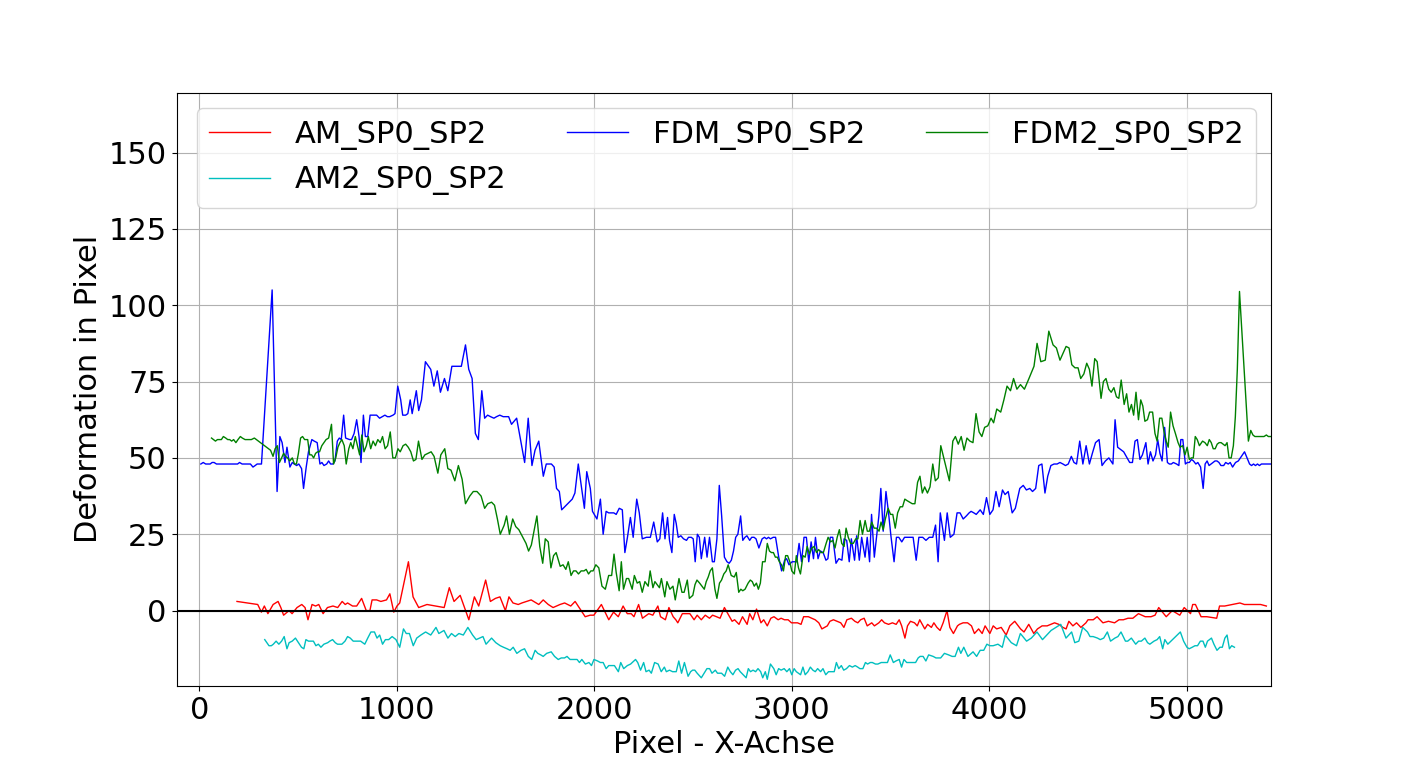
\includegraphics[width=0.95\textwidth]{images/compare_materials.png}
  \caption{Vergleich von Materialien und Bauteilgeometrien}
  \label{fig:materials}
\end{figure}

In dieser Validierung wurden nur 
die äußeren Randgeometrien verglichen. Die Deformationen der inneren 
Geometrien der Bauteile ist sehr ähnlich zu dem äußeren Verhalten und passt 
auch zu dem erwarteten Verhalten der Bauteile.

\section{Limitierung der Deformationerkennung} \label{limits}

Grundsätzlich funktioniert die Deformationserkennung, wie schon angesprochen kann es 
jedoch vorkommen, dass die erkannte Deformation nicht den korrekten Werten entspricht.
Fehler im Stitching Prozess können zu starken Änderungen in der Deformationserkennung führen. 
Wie in Abbildung~\ref{fig:errors} zu sehen ist, kann sich die Höhe des Bauteils 
zwischen zwei Spannungsstufen unterscheiden. Er ist erkennbar, dass der Rand der einen 
Kontur, repräsentiert durch die magenta gefärbte Linie, immer größer ist als 
der Rand der anderen Kontur, hier in blau dargestellt.
Dieser Versatz entsteht, weil beim Stitching eine Transformation verwendet wurde die um 
wenige Pixel versetzt ist. Dadurch wächst die erkannte Deformation.
Aus diesem Grund existieren in den Abbildungen \ref{fig:am_defos} und \ref{fig:fdm_defos}
Linien die nicht dem erwarteten Verhalten entsprechen.
In Abbildung \ref{fig:fdm_defos} zum Beispiel, sollte die Deformation zwischen den 
Spannungsstufen eins und zwei 
(in rot dargestellt) am kleinsten sein. Stattdessen liegt die Kurve bei -50 Pixeln im Graph 
und nicht nahe der Nulllinie.
Trotz Fehler in der Position der Deformationskurve, ist der Verlauf aussagekräftig und zeigt an, 
wie sich die Deformation im Verlauf des Bauteils verändert hat.

\begin{figure}[H]
  \centering
  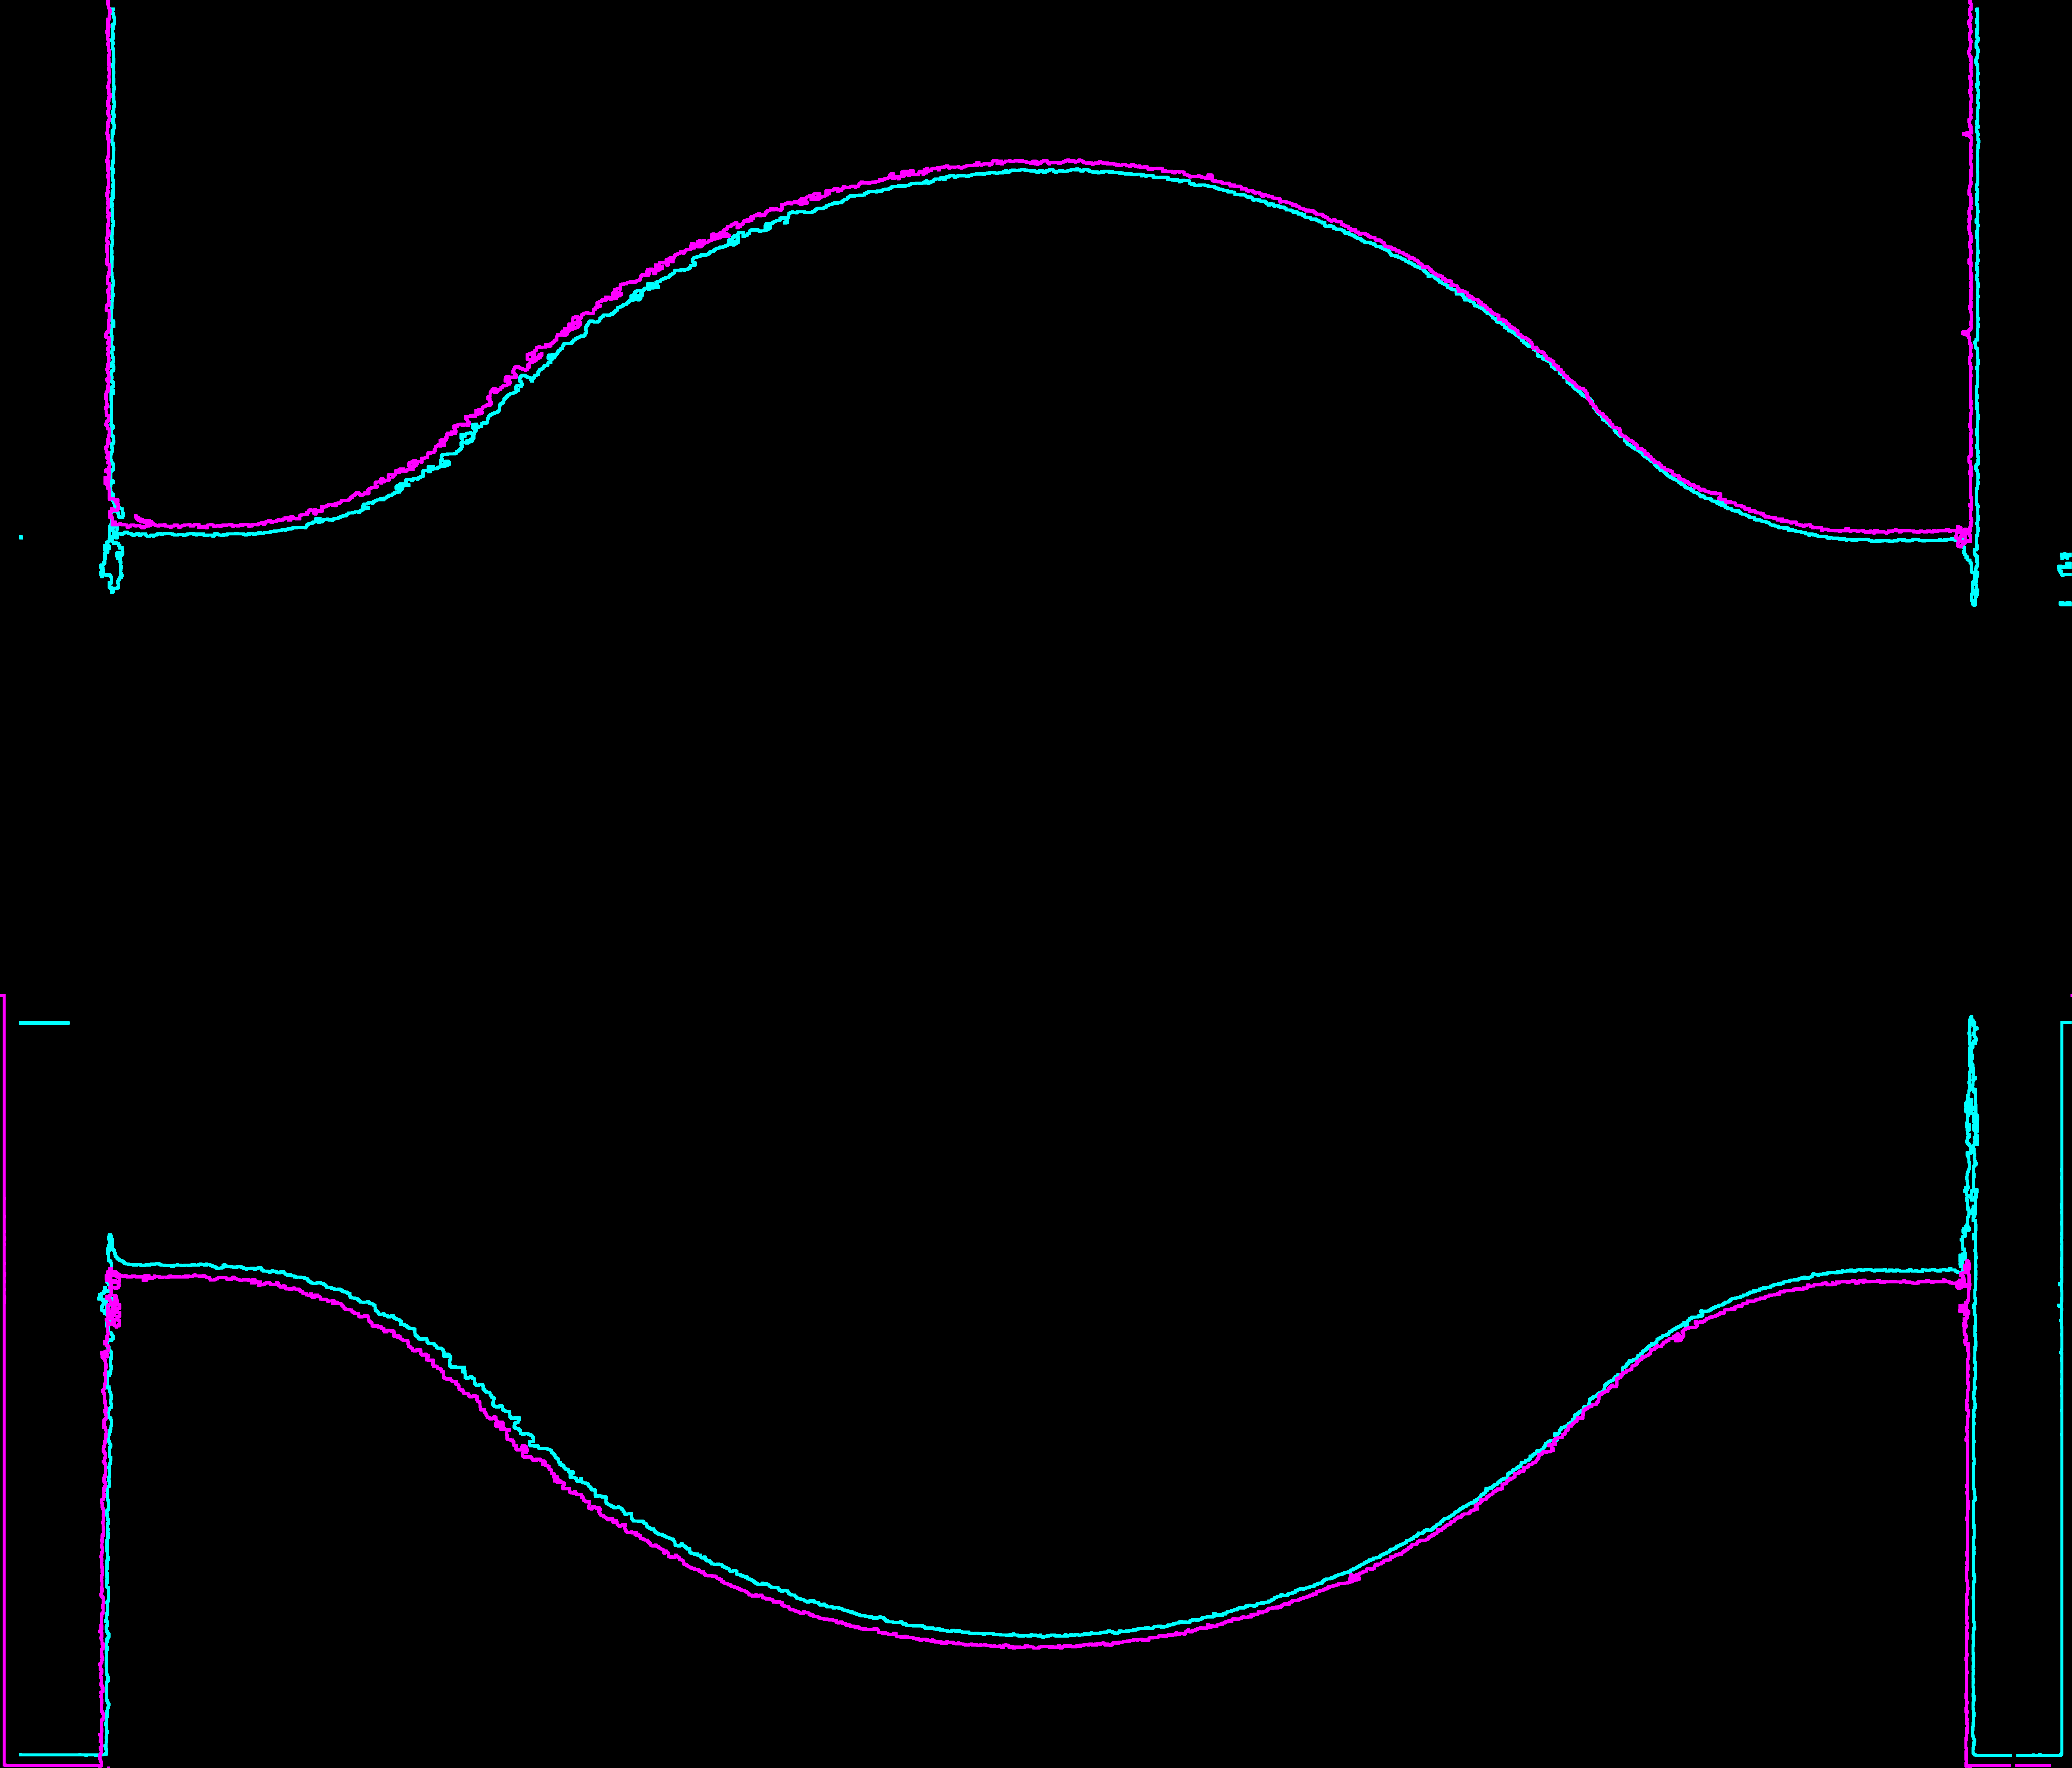
\includegraphics[width=0.95\textwidth]{images/contours_matching_36.png}
  \caption{Vergleich von Konturen aus nicht korrekt zusammengefügten Bildern.}
  \label{fig:errors}
\end{figure}

Zusätzlich kann bei Bildern ohne klare Konturen, das Stitching nicht korrekt durchgeführt
werden. Dies ist bei additiv gefertigten Metallbauteilen mit Stützstruktur der Fall.
In Abbildung \ref{fig:am_parts} (a) ist ein solches Teil dargestellt. 
Das Bild, das aus dem Scan dieses Bauteils erstellt wurde, 
ist in Abbildung \ref{fig:errorimage} zu sehen. Es lassen sich keine eindeutigen Konturen 
erkennen, die für das Stitching genutzt werden könnten. Aus diesem Grund schlägt das Stitching 
fehl und es kann keine Deformationsanalyse durchgeführt werden.

\begin{figure}[H]
  \centering
  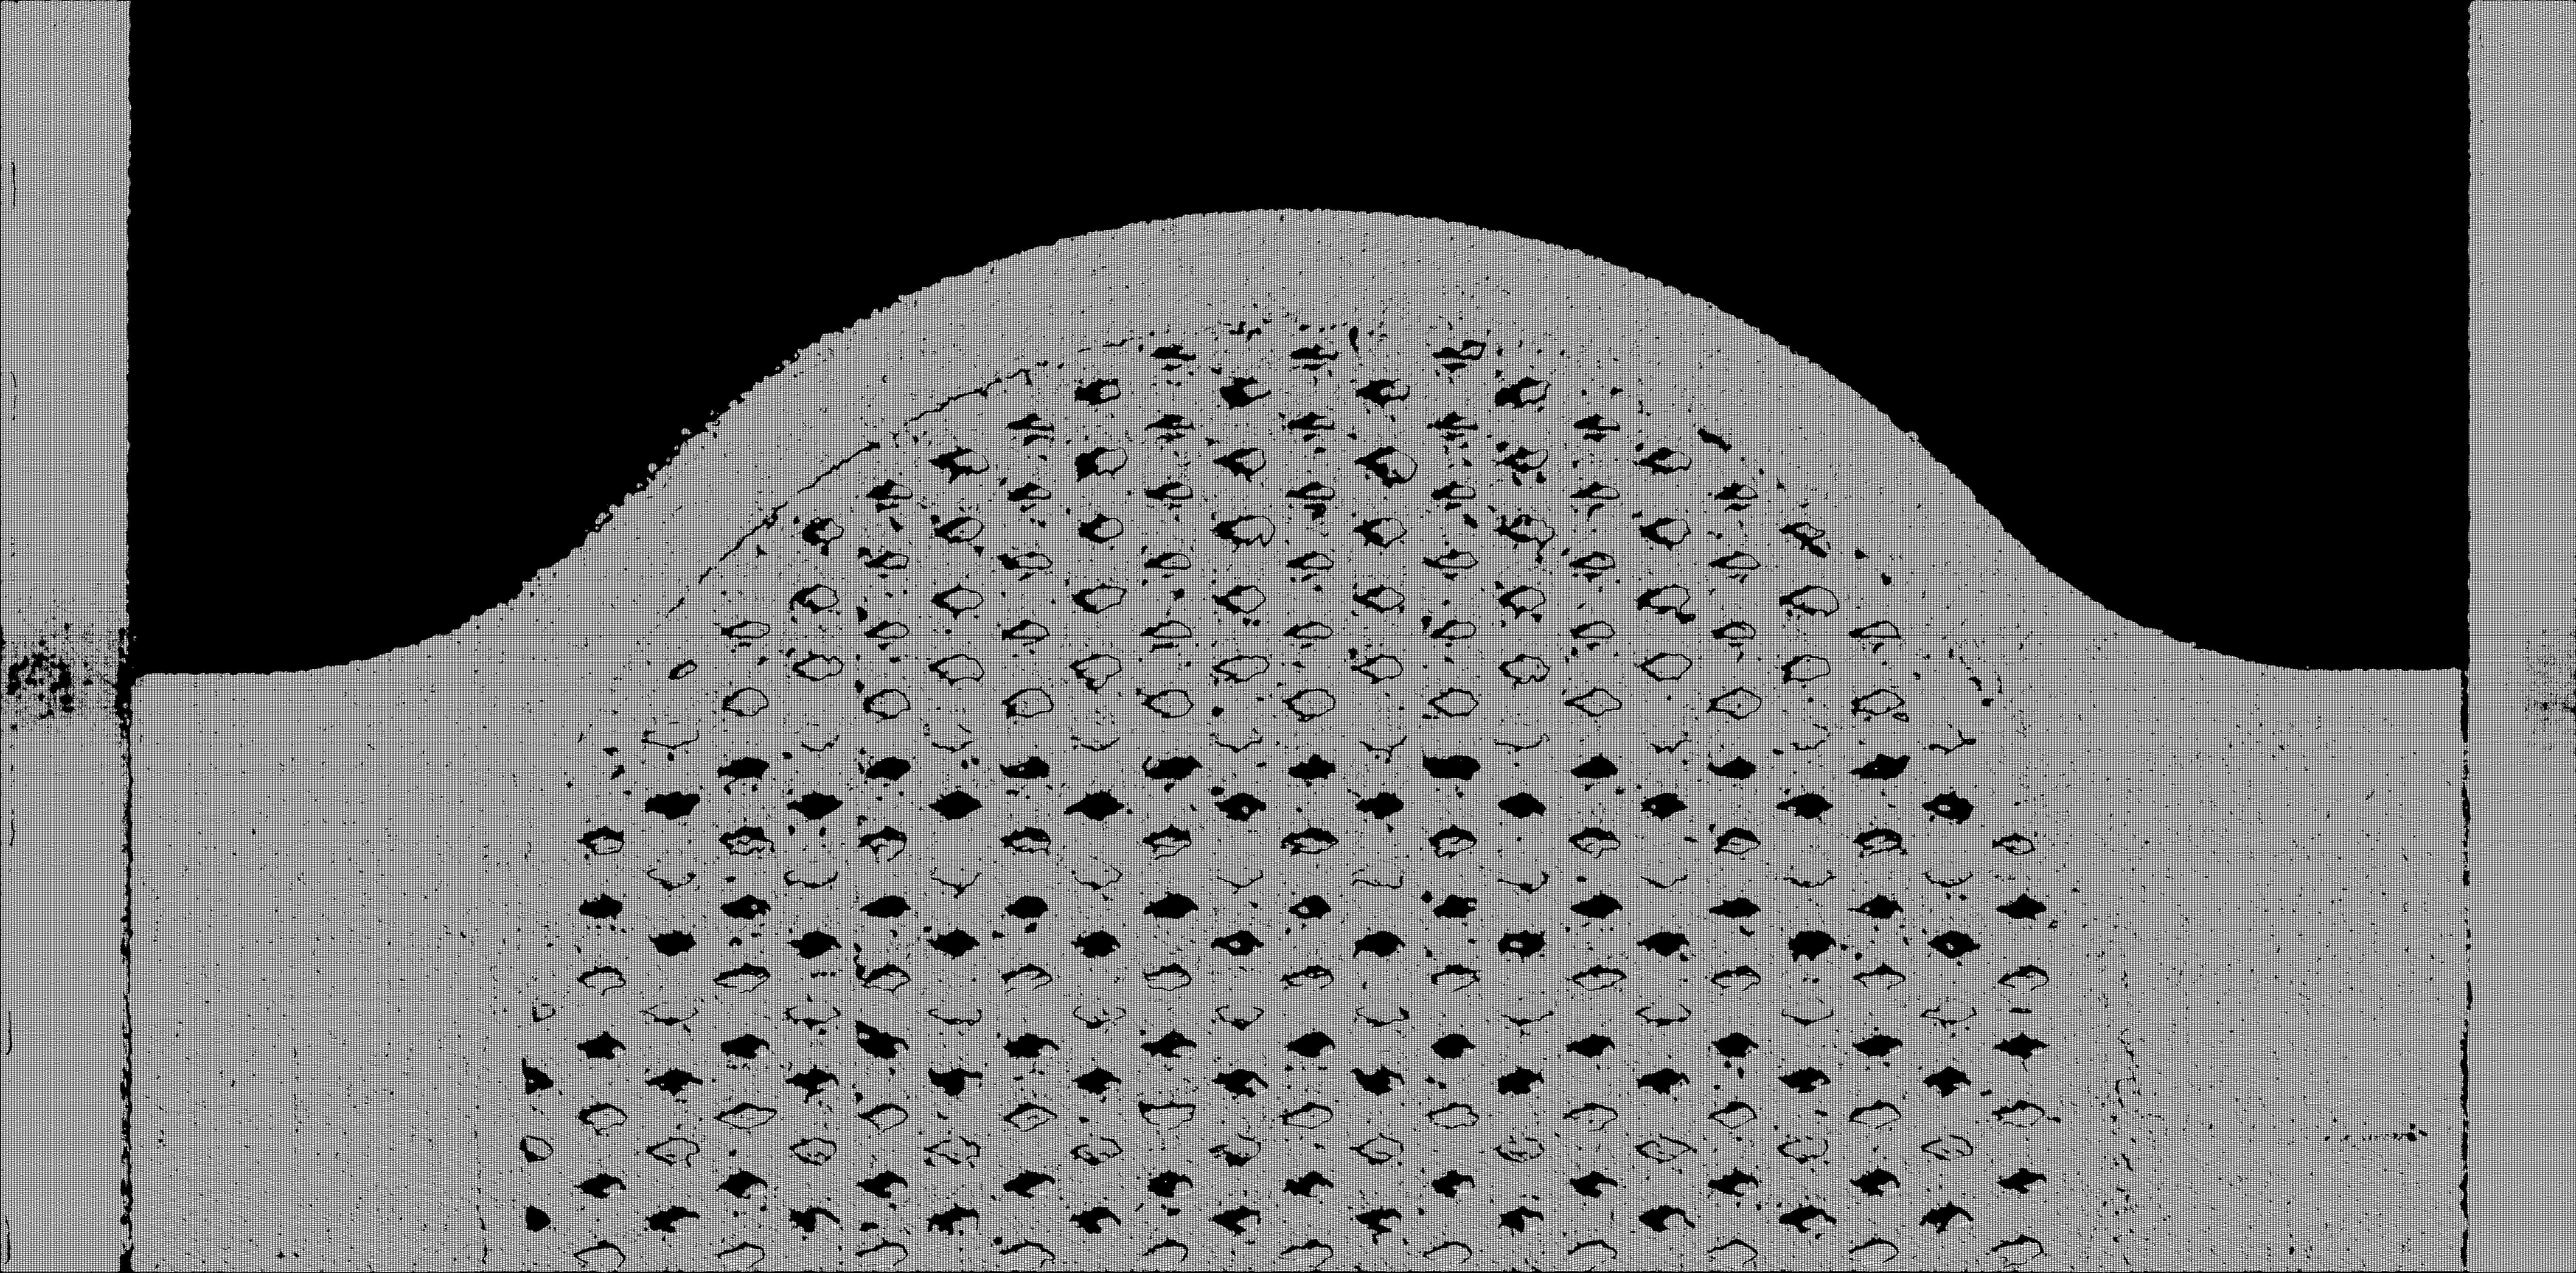
\includegraphics[width=0.95\textwidth]{images/am0.png}
  \caption{Bild eines Scans von einem Metallbauteil mit Stützstruktur.}
  \label{fig:errorimage}
\end{figure}


